\documentclass{beamer}
\usetheme{default}
\beamertemplatenavigationsymbolsempty

\usepackage{fontspec}
\setmainfont{Linux Libertine}
\setsansfont{Linux Biolinum}


\usepackage[spanish]{babel}
\usepackage{tikz}
\usetikzlibrary{babel}
\usepackage{siunitx}
\usepackage{physics}
\usepackage{color}
\usepackage{unicode-math}

\newcommand{\sub}[1]{ _{{\scriptscriptstyle \mathit{#1}}}  }
\newcommand{\kb}{k\sub{B}}

\definecolor{PlotDefault}{HTML}{64B5CD}
\definecolor{PlotSecondary}{HTML}{CCB974}
\definecolor{NiceBlack}{HTML}{444444}

\definecolor{NiceBlue}{HTML}{64B5CD}
\definecolor{NiceRed}{HTML}{C44E52}
\definecolor{NiceYellow}{HTML}{CCB974}

\definecolor{SpinUp}{HTML}{226AB2}
\definecolor{SpinDown}{HTML}{B22222}

\definecolor{tw1_1e4}{HTML}{64B5CD}
\definecolor{tw1_1e5}{HTML}{98B7A0}
\definecolor{tw1_1e6}{HTML}{CBB873}
\definecolor{tw1_1e7}{HTML}{C78262}
\definecolor{tw1_1e8}{HTML}{C44E52}

\usepackage{mathrsfs}
\newcommand{\Ham}{\mathscr{H}}

\begin{document}

\begin{frame}
  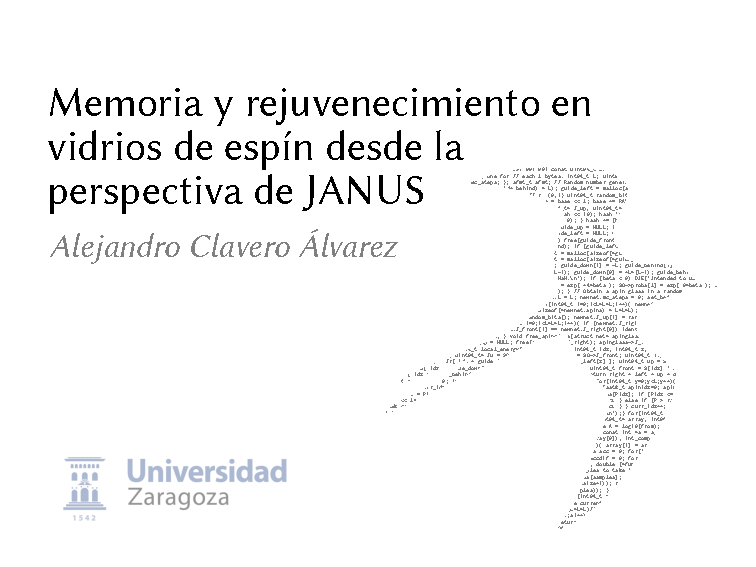
\includegraphics[width=\textwidth]{images/beamer_title.pdf}
\end{frame}


\begin{frame}
  \frametitle{¿Qué es un vidrio de espín?}

    \pause

  \begin{columns}


    \column{0.33\textwidth}

    \begin{center}
      \begin{tikzpicture}[scale=0.5]
        \node at (1,1) {\textcolor{SpinUp}{↑}};
        \node at (1,2) {\textcolor{SpinUp}{↑}};
        \node at (1,3) {\textcolor{SpinUp}{↑}};
        \node at (1,4) {\textcolor{SpinUp}{↑}};
        \node at (1,5) {\textcolor{SpinUp}{↑}};
        \node at (2,1) {\textcolor{SpinUp}{↑}};
        \node at (2,2) {\textcolor{SpinUp}{↑}};
        \node at (2,3) {\textcolor{SpinUp}{↑}};
        \node at (2,4) {\textcolor{SpinUp}{↑}};
        \node at (2,5) {\textcolor{SpinUp}{↑}};
        \node at (3,1) {\textcolor{SpinUp}{↑}};
        \node at (3,2) {\textcolor{SpinUp}{↑}};
        \node at (3,3) {\textcolor{SpinUp}{↑}};
        \node at (3,4) {\textcolor{SpinUp}{↑}};
        \node at (3,5) {\textcolor{SpinUp}{↑}};
        \node at (4,1) {\textcolor{SpinUp}{↑}};
        \node at (4,2) {\textcolor{SpinUp}{↑}};
        \node at (4,3) {\textcolor{SpinUp}{↑}};
        \node at (4,4) {\textcolor{SpinUp}{↑}};
        \node at (4,5) {\textcolor{SpinUp}{↑}};
        \node at (5,1) {\textcolor{SpinUp}{↑}};
        \node at (5,2) {\textcolor{SpinUp}{↑}};
        \node at (5,3) {\textcolor{SpinUp}{↑}};
        \node at (5,4) {\textcolor{SpinUp}{↑}};
        \node at (5,5) {\textcolor{SpinUp}{↑}};
      \end{tikzpicture}
    \end{center}

    \begin{center}
      \textsc{Ferromagnetismo}
    \end{center}

    \pause

    \column{0.33\textwidth}

    \begin{center}
      \begin{tikzpicture}[scale=0.5]
        \node at (1,1) {\textcolor{SpinUp}{↑}};
        \node at (1,2) {\textcolor{SpinDown}{↓}};
        \node at (1,3) {\textcolor{SpinUp}{↑}};
        \node at (1,4) {\textcolor{SpinDown}{↓}};
        \node at (1,5) {\textcolor{SpinUp}{↑}};
        \node at (2,1) {\textcolor{SpinDown}{↓}};
        \node at (2,2) {\textcolor{SpinUp}{↑}};
        \node at (2,3) {\textcolor{SpinDown}{↓}};
        \node at (2,4) {\textcolor{SpinUp}{↑}};
        \node at (2,5) {\textcolor{SpinDown}{↓}};
        \node at (3,1) {\textcolor{SpinUp}{↑}};
        \node at (3,2) {\textcolor{SpinDown}{↓}};
        \node at (3,3) {\textcolor{SpinUp}{↑}};
        \node at (3,4) {\textcolor{SpinDown}{↓}};
        \node at (3,5) {\textcolor{SpinUp}{↑}};
        \node at (4,1) {\textcolor{SpinDown}{↓}};
        \node at (4,2) {\textcolor{SpinUp}{↑}};
        \node at (4,3) {\textcolor{SpinDown}{↓}};
        \node at (4,4) {\textcolor{SpinUp}{↑}};
        \node at (4,5) {\textcolor{SpinDown}{↓}};
        \node at (5,1) {\textcolor{SpinUp}{↑}};
        \node at (5,2) {\textcolor{SpinDown}{↓}};
        \node at (5,3) {\textcolor{SpinUp}{↑}};
        \node at (5,4) {\textcolor{SpinDown}{↓}};
        \node at (5,5) {\textcolor{SpinUp}{↑}};
      \end{tikzpicture}
    \end{center}

    \begin{center}
      \textsc{Antiferromagnetismo}
    \end{center}

    \pause

    \column{0.33\textwidth}

    \begin{center}
      \begin{tikzpicture}[scale=0.5]
        \node at (1,1) {\textcolor{SpinDown}{↓}};
        \node at (1,2) {\textcolor{SpinDown}{↓}};
        \node at (1,3) {\textcolor{SpinDown}{↓}};
        \node at (1,4) {\textcolor{SpinUp}{↑}};
        \node at (1,5) {\textcolor{SpinDown}{↓}};
        \node at (2,1) {\textcolor{SpinUp}{↑}};
        \node at (2,2) {\textcolor{SpinUp}{↑}};
        \node at (2,3) {\textcolor{SpinUp}{↑}};
        \node at (2,4) {\textcolor{SpinUp}{↑}};
        \node at (2,5) {\textcolor{SpinDown}{↓}};
        \node at (3,1) {\textcolor{SpinDown}{↓}};
        \node at (3,2) {\textcolor{SpinDown}{↓}};
        \node at (3,3) {\textcolor{SpinUp}{↑}};
        \node at (3,4) {\textcolor{SpinUp}{↑}};
        \node at (3,5) {\textcolor{SpinUp}{↑}};
        \node at (4,1) {\textcolor{SpinUp}{↑}};
        \node at (4,2) {\textcolor{SpinUp}{↑}};
        \node at (4,3) {\textcolor{SpinDown}{↓}};
        \node at (4,4) {\textcolor{SpinDown}{↓}};
        \node at (4,5) {\textcolor{SpinUp}{↑}};
        \node at (5,1) {\textcolor{SpinDown}{↓}};
        \node at (5,2) {\textcolor{SpinDown}{↓}};
        \node at (5,3) {\textcolor{SpinUp}{↑}};
        \node at (5,4) {\textcolor{SpinDown}{↓}};
        \node at (5,5) {\textcolor{SpinUp}{↑}};
      \end{tikzpicture}
    \end{center}

    \begin{center}
      \textsc{Vidrio de espín}
    \end{center}

  \end{columns}

\end{frame}


\begin{frame}
  \frametitle{Dip experiment protocol}
  \begin{center}
    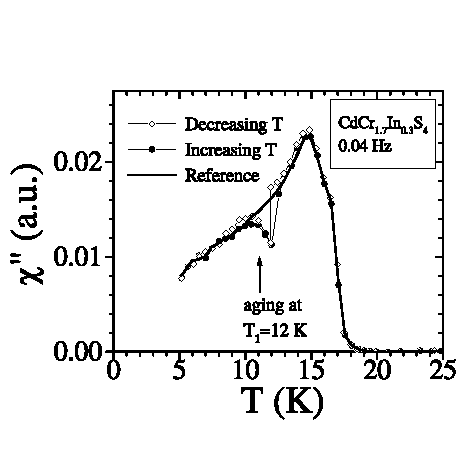
\includegraphics{images/dip_full.pdf}
  \end{center}
\end{frame}

\begin{frame}
  \frametitle{Dip experiment protocol}
  \begin{center}
    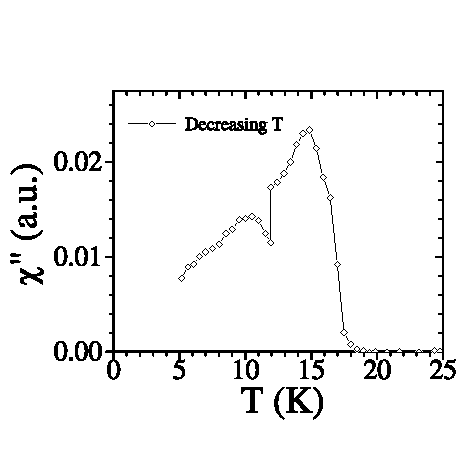
\includegraphics{images/dip_onlydecrease.pdf}
  \end{center}
\end{frame}

\begin{frame}
  \frametitle{Dip experiment protocol}
  \begin{center}
    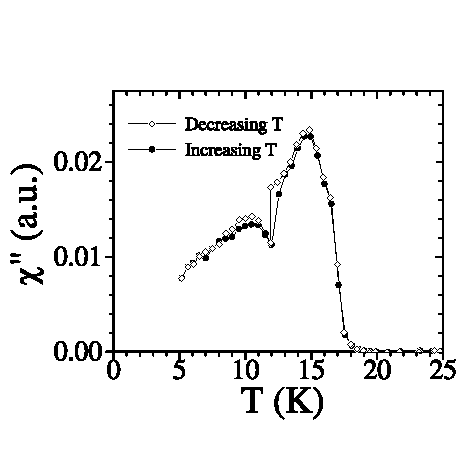
\includegraphics{images/dip_noref.pdf}
  \end{center}
\end{frame}

\begin{frame}
  \frametitle{Dip experiment protocol}
  \begin{center}
    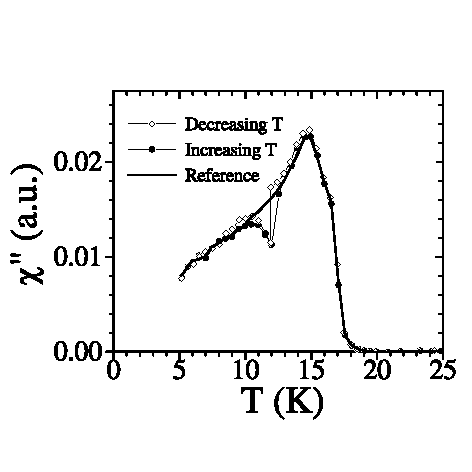
\includegraphics{images/dip_abridged.pdf}
  \end{center}
\end{frame}

\begin{frame}
  \frametitle{Protocolo de dos temperaturas}
  \begin{center}
    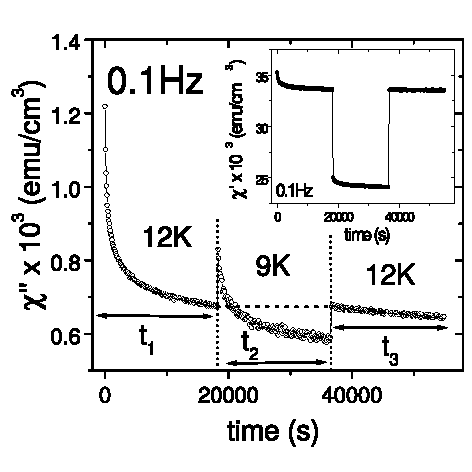
\includegraphics{images/threetempsprotocol_full.pdf}
  \end{center}
\end{frame}

\begin{frame}
  \frametitle{Protocolo de dos temperaturas}
  \begin{center}
    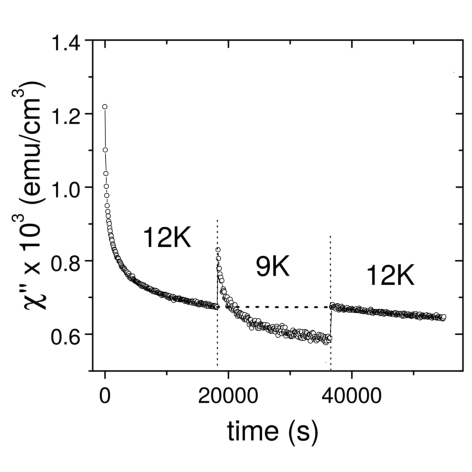
\includegraphics{images/threetempsprotocol_abridged.pdf}
  \end{center}
\end{frame}

\begin{frame}
  \frametitle{Protocolo de dos temperaturas}
  \begin{center}
    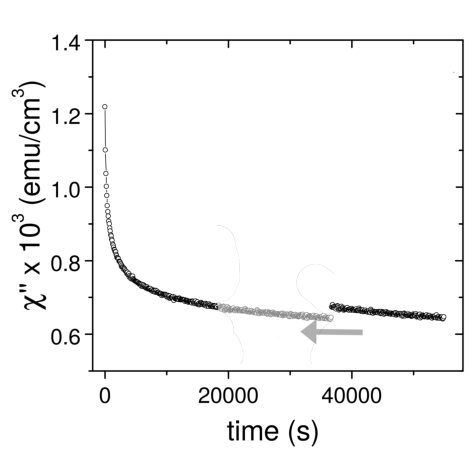
\includegraphics{images/threetempsprotocol_empalma.pdf}
  \end{center}
\end{frame}

\begin{frame}
  \frametitle{Protocolo de dos temperaturas}
  \begin{center}
    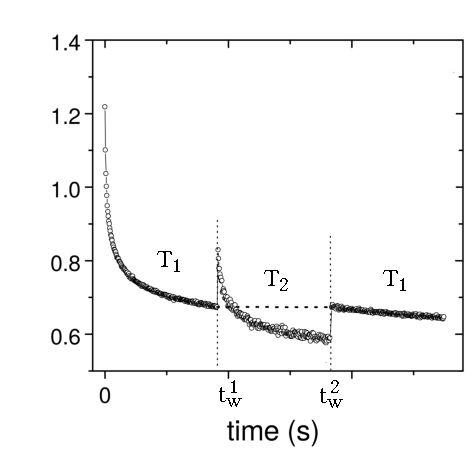
\includegraphics{images/threetempsprotocol_defs.pdf}
  \end{center}
\end{frame}


\begin{frame}
  \frametitle{Modelo}

  \pause

  \begin{columns}

    \column{0.5\textwidth}

    \begin{equation*}
      J(r) \ ∝ \ \frac{\cos(2K\sub{F} r)}{r^3}
    \end{equation*}

    \pause

    \begin{equation*}
      \Ham \ = \  - \sum_{\expval{i,j}} J_{ij} s_i s_j
    \end{equation*}

    \pause

    \column{0.5\textwidth}

    \begin{center}
      \includegraphics{images/EAfigure.pdf}
    \end{center}

  \end{columns}

\end{frame}

\begin{frame}
  \frametitle{Modelo}
  \begin{center}
    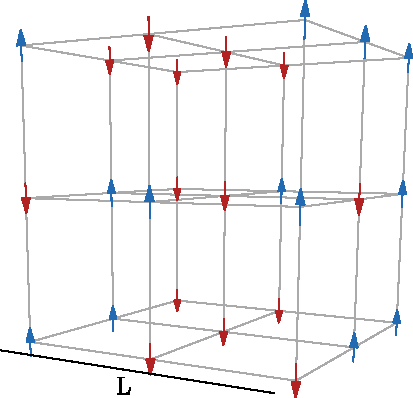
\includegraphics{../study_cases/gridplot/gridplot.pdf}
  \end{center}
\end{frame}

\begin{frame}
  \frametitle{Magnitudes}
  \pause
% E,  M→q, C, χ, C₄
  \begin{center}
    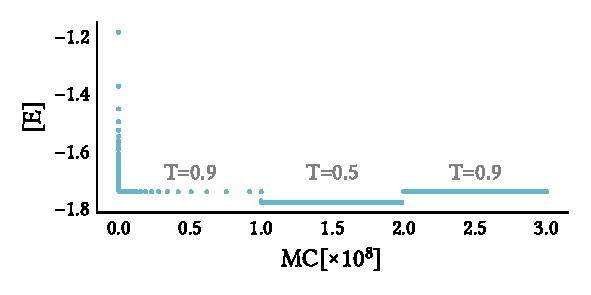
\includegraphics{../study_cases/energy_in_protocol/energyprotocol_beamer.pdf}
  \end{center}
    \begin{equation*}
      E \ = \  - \sum_{\expval{i,j}} J_{ij} s_i s_j
    \end{equation*}
\end{frame}

\begin{frame}
  \frametitle{Magnitudes}
% E,  M→q, C, χ, C₄
  \begin{center}
    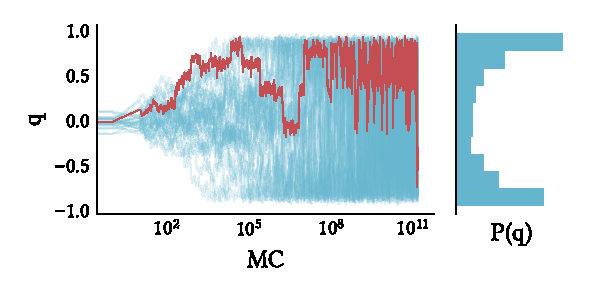
\includegraphics{../study_cases/overlap/overlap_beamer.pdf}
  \end{center}
  \begin{equation*}
    q = \frac{1}{V} \sum_{i} s_i^a s_i^b
  \end{equation*}
\end{frame}


\begin{frame}
  \frametitle{Magnitudes}
% E,  M→q, C, χ, C₄
  \begin{center}
    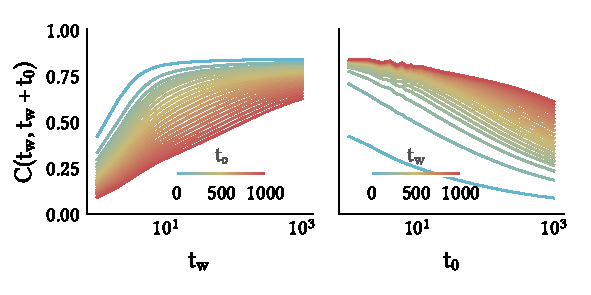
\includegraphics{../study_cases/corr_functional_dependence/corrfunction_beamer.pdf}
  \end{center}
  \begin{equation*}
    C(t_w, t_w + t₀) \ = \  \frac{1}{V} \sum_{i} \expval{s_i(t_w) ⋅ s_i(t_w+t₀)}
  \end{equation*}
\end{frame}


\begin{frame}
  \frametitle{Magnitudes}
% E,  M→q, C, χ, C₄
  \begin{center}
    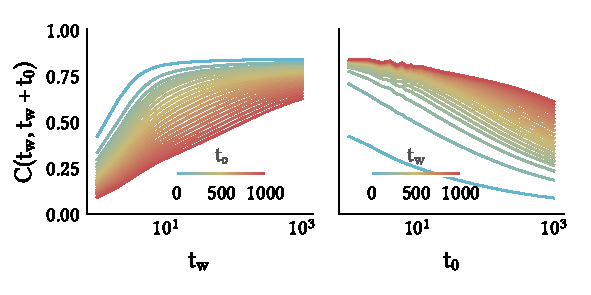
\includegraphics{../study_cases/corr_functional_dependence/corrfunction_beamer.pdf}
  \end{center}
  \begin{equation*}
    C(t_w, t_w + t₀) \ \rightarrow \ \ \ \boxed{\chi = \beta(1-C)}
  \end{equation*}
\end{frame}

\begin{frame}
  \frametitle{Rejuvenecimiento}
  \pause
  \begin{center}
    \begin{tikzpicture}
      \node at (7,3) {{\large \textsc{Fuerte}}};
      % Axis
      \draw[NiceBlack] (0,0) -- (10,0) node [below, NiceBlack] {$t_w$};
      \draw[NiceBlack] (0,0) -- (0,4) node [left, NiceBlack] {$χ$};
      % Curves
      \draw[ultra thick, PlotDefault] (0.5,4) to[out=-90, in=170] (3,1);
      \draw[ultra thick, dashed, PlotDefault!60!white] (3,1) to[out=-10,
      in=175] (6,0.6); % Extension
      \draw[ultra thick, PlotDefault] (6,1) to[out=-10, in=175] (9,0.6);
      \draw[ultra thick, PlotSecondary] (3,2) to[out=-85, in=180]
      (6,0.5);
    \end{tikzpicture}
  \end{center}
\end{frame}

\begin{frame}
  \frametitle{Rejuvenecimiento}
  \begin{center}
    \begin{tikzpicture}
      \node at (7,3) {{\large \textsc{Fuerte}}};
      % Axis
      \draw[NiceBlack] (0,0) -- (10,0) node [below, NiceBlack] {$t_w$};
      \draw[NiceBlack] (0,0) -- (0,4) node [left, NiceBlack] {$χ$};
      % help lines
      \draw[thin, black!20!white] (3,2) -- (3,0);
      \draw[thin, black!20!white] (3.8,0.85) -- (3.8,0);
      \draw[thin, black!20!white] (3,2) -- (1.2,2);
      \draw[thin, black!20!white] (1.2,2) -- (1.2,0);
      % Curves
      \draw[ultra thick, PlotDefault] (0.5,4) to[out=-90, in=170] (3,1);
      \draw[ultra thick, dashed, PlotDefault!60!white] (3,1) to[out=-10,
      in=175] (6,0.6); % Extension
      \draw[ultra thick, PlotDefault] (6,1) to[out=-10, in=175] (9,0.6);
      \draw[ultra thick, PlotSecondary] (3,2) to[out=-85, in=180]
      (6,0.5);
      % measures
      \fill[gray] (1.2,0) circle (0.1) node[below, NiceBlack]
      {$t_\mathit{rej}^L$};
      \draw[<->, NiceBlack] (1.2,2) -- (3,2) node[midway, above,
      NiceBlack] {$Δt_\mathit{rej}^L$};
      \draw[<->, NiceBlack] (3.0,2) -- (3.0,1) node[midway, left,
      NiceBlack] {$Δχ$};
      \draw[<->, NiceBlack] (3,-0.2) -- (3.8,-0.2) node[midway, below,
      NiceBlack] {$t_\mathit{rej}^A$};
    \end{tikzpicture}
  \end{center}
\end{frame}

\begin{frame}
  \frametitle{Rejuvenecimiento}
  \begin{center}
    \begin{tikzpicture}
      \node at (7,3) {{\large \textsc{Débil}}};
      % Axis
      \draw[NiceBlack] (0,0) -- (10,0) node [below, NiceBlack] {$t_w$};
      \draw[NiceBlack] (0,0) -- (0,4) node [left, NiceBlack] {$χ$};
      % help lines
      \draw[thin, black!20!white] (3,2) -- (3,0);
      % Curves
      \draw[ultra thick, PlotDefault] (0.5,4) to[out=-90, in=170] (3,1);
      \draw[ultra thick, dashed, PlotDefault!60!white] (3,1) to[out=-10,
      in=175] (6,0.6); % Extension
      \draw[ultra thick, PlotDefault] (6,1) to[out=-10, in=175] (9,0.6);
      \draw[ultra thick, PlotSecondary] (3,0.50) to[out=-25, in=180]
      (6,0.1);
      % measures
      \draw[<->, NiceBlack] (3.0,0.5) -- (3.0,1) node[midway, left,
      NiceBlack] {$Δχ$};
    \end{tikzpicture}
  \end{center}
\end{frame}

\begin{frame}
  \frametitle{Rejuvenecimiento}
  \begin{center}
    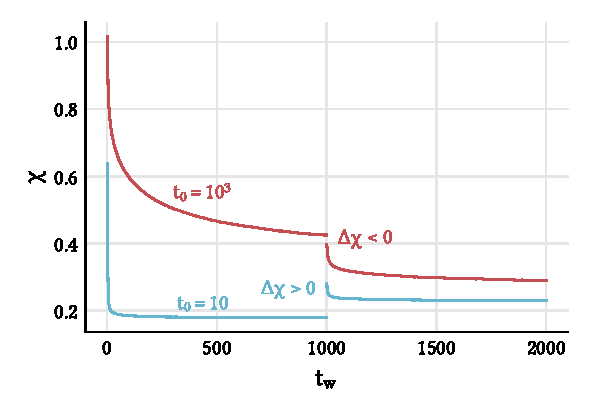
\includegraphics{../study_cases/vanishingrejuvenation/trej_A_beamer.pdf}
  \end{center}
\end{frame}

\begin{frame}
  \frametitle{Rejuvenecimiento}
  \begin{center}
    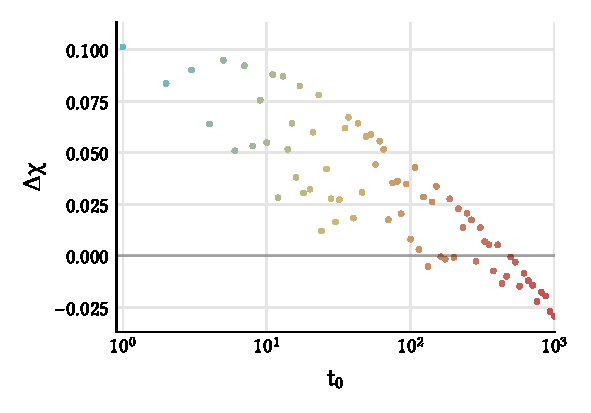
\includegraphics{../study_cases/vanishingrejuvenation/trej_B_beamer.pdf}
  \end{center}
\end{frame}

\begin{frame}
  \frametitle{Rejuvenecimiento}
  \begin{center}
    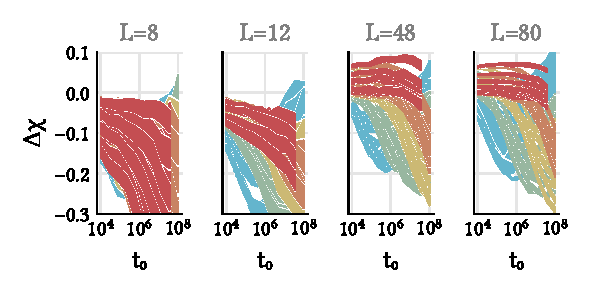
\includegraphics[width=\textwidth]{../study_cases/trejanalysis/nonaveraged_forbeamer.pdf}
  \end{center}
  \Large $t_w^1$: \quad
  $10^4$ (\textcolor{tw1_1e4}{●}), \ \
  $10^5$ (\textcolor{tw1_1e5}{●}), \ \
  $10^6$ (\textcolor{tw1_1e6}{●}), \ \
  $10^7$ (\textcolor{tw1_1e7}{●}), \ \
  $10^8$ (\textcolor{tw1_1e8}{●})
\end{frame}

\begin{frame}
  \frametitle{Rejuvenecimiento}
  \begin{center}
    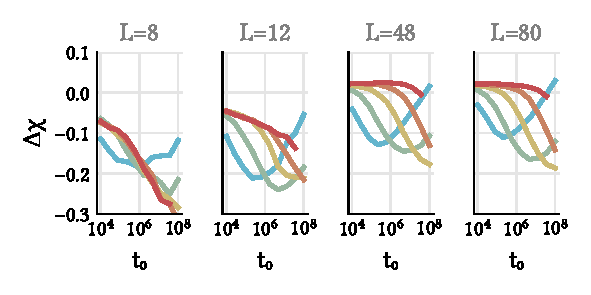
\includegraphics[width=\textwidth]{../study_cases/trejanalysis/averaged_forbeamer.pdf}
  \end{center}
  \Large $t_w^1$: \quad
  $10^4$ (\textcolor{tw1_1e4}{●}), \ \
  $10^5$ (\textcolor{tw1_1e5}{●}), \ \
  $10^6$ (\textcolor{tw1_1e6}{●}), \ \
  $10^7$ (\textcolor{tw1_1e7}{●}), \ \
  $10^8$ (\textcolor{tw1_1e8}{●})
\end{frame}

\begin{frame}
  \frametitle{Rejuvenecimiento}
  \begin{center}
    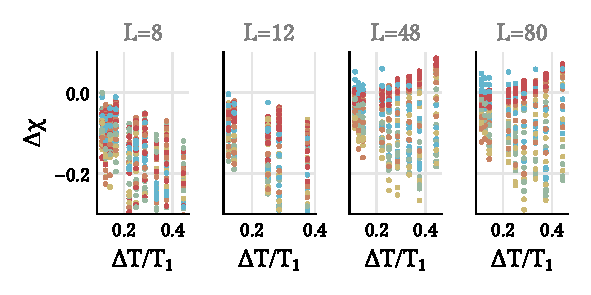
\includegraphics[width=\textwidth]{../study_cases/trejanalysis/temps_forbeamer.pdf}
  \end{center}
  \Large $t_w^1$: \quad
  $10^4$ (\textcolor{tw1_1e4}{●}), \ \
  $10^5$ (\textcolor{tw1_1e5}{●}), \ \
  $10^6$ (\textcolor{tw1_1e6}{●}), \ \
  $10^7$ (\textcolor{tw1_1e7}{●}), \ \
  $10^8$ (\textcolor{tw1_1e8}{●})
\end{frame}

\begin{frame}
  \frametitle{Memoria}
  \pause
  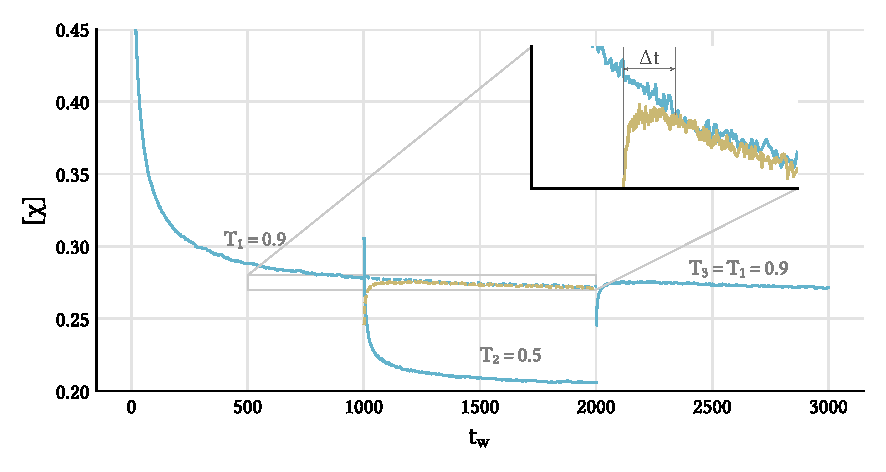
\includegraphics[width=\textwidth]{../study_cases/memory_toy/memorytoy_handedit.pdf}
\end{frame}

\begin{frame}
  \frametitle{Memoria}
  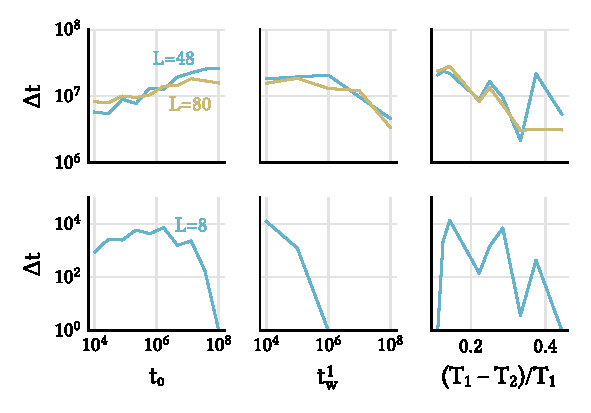
\includegraphics{../study_cases/memory/dependences_beamer_handedit.pdf}
\end{frame}

\begin{frame}
  \frametitle{Conclusiones}
  \begin{itemize}
  \item Dificultad computacional
  \item Problemas técnicos, planificación
  \item Rejuvenecimiento débil
  \item Memoria robusta
  \end{itemize}

\vfill
\hfill
\textcolor{gray}{\textit{Agradecimientos a BIFI y Janus Collaboration}}

\end{frame}

\begin{frame}

\end{frame}


\end{document}
